\documentclass[11pt,a4paper]{article}

\usepackage[margin=2.4cm]{geometry}
\usepackage{graphicx}
\usepackage{booktabs}
\usepackage{amsmath}
\usepackage{amssymb}
\usepackage{xcolor}
\usepackage{caption}
\usepackage{enumitem}
\usepackage[hidelinks]{hyperref}
\usepackage{tabularx}

\graphicspath{{figures/}}
\captionsetup{font=small,labelfont=bf}

\definecolor{accent}{RGB}{140,21,21}
\definecolor{softgray}{RGB}{245,245,245}

\newcommand{\term}[1]{\textbf{\textcolor{accent}{#1}}}
\newcommand{\code}[1]{\texttt{\small #1}}

\title{\vspace{-1.2cm}\textbf{Credit Card Fraud Detection:\\
A Comparative Study of Classical ML, Deep Learning,\\ Generative Oversampling, Ensembles and Graph Neural Networks}\\[0.4cm]
\large With a self-contained introduction to machine-learning model families\\[0.6cm]}
\author{Divya \\ Indian Institute of Technology Hyderabad}
\date{\today}

\begin{document}
\maketitle

\begin{abstract}
\noindent
We build and rigorously evaluate a complete fraud-detection pipeline on the public Kaggle ULB
credit-card dataset (284{,}807 transactions, 492 frauds, $0.173\%$ prevalence).
Seventy-two experiments span five model families --- linear models, tree ensembles,
neural networks, generative-augmentation pipelines, and graph neural networks --- combined with
seven imbalance-handling strategies, all under one deployment-honest protocol:
a chronological 70/15/15 train/validation/test split, validation-only tuning,
and a test set that keeps its natural imbalance.
The champion, a Random Forest trained on SMOTE-ENN-resampled data, reaches
$\text{PR-AUC} = 0.795$ ($F_1 = 0.848$, MCC $= 0.855$, one false positive in 42{,}722 transactions),
the top of the honest-protocol range reported in recent literature.
Nine controlled ablations explain \emph{why}: hybrid sampling wins for trees;
naive extreme class weighting silently collapses boosted models; cross-family
ensembling helps while seed averaging does not; depth does not help on PCA features;
and shuffling the split inflates scores by up to $+0.06$, reproducing the numbers
that dominate older literature. Stratified bootstrap analysis shows all models are
statistical ties at this test size --- the contribution is the protocol and the analysis,
not a leaderboard winner. Every prediction is explained with SHAP, whose feature
attributions independently confirm the exploratory analysis.
The report doubles as a self-contained tutorial: each model family is introduced from
first principles before its experimental results are discussed.
\end{abstract}

\newpage
\tableofcontents
\newpage

% ============================================================================
\section{Introduction}
% ============================================================================

Card-not-present fraud costs the payments industry tens of billions of dollars annually,
and every fraudulent transaction that slips through is a direct loss while every legitimate
transaction that is wrongly blocked damages customer trust. Machine-learning classifiers sit
at the heart of modern fraud engines: they score each incoming transaction, and a policy layer
decides whether to approve, challenge, or block.

This project builds such a scoring system end-to-end and asks three questions:

\begin{enumerate}[leftmargin=*]
      \item \textbf{Which model family} detects fraud best when the evaluation is done honestly?
      \item \textbf{How should extreme class imbalance} (one fraud per 578 legitimate transactions)
            be handled --- resampling, cost re-weighting, synthetic generation, or anomaly detection?
      \item \textbf{How much do methodology choices} (split protocol, tuning discipline,
            uncertainty reporting) change the conclusions?
\end{enumerate}

The project is also written as a \term{learning document}. Section~\ref{sec:taxonomy}
introduces every model family from first principles so that a reader new to machine learning
can follow exactly what was trained and why. All 72 experiments, including failures, are
logged in the accompanying experiment inventory, and every design decision is backed by a
controlled ablation rather than a citation.

\subsection{Reference studies: what they do, what they report, where we land}
\label{sec:refstudies}
Before any result is presented, Table~\ref{tab:refpos} fixes the comparison set. Every figure
below was read from the cited paper, and each is paired with the number from this study that is
actually comparable to it --- matching \emph{protocol} first, model second, because
Section~\ref{sec:splittab} shows protocol dominates.

\begin{table}[h]
      \centering\small
      \caption{Verified published reference points and the comparable result from this work.
      PR-AUC throughout. The only protocol-matched row --- chronological versus chronological
      --- is the first.}
      \label{tab:refpos}
      \begin{tabularx}{\textwidth}{lXlll}
            \toprule
            Study & Protocol / data & Theirs & Ours & $\Delta$\\
            \midrule
            Sang 2026~\cite{eai2026} & ULB, \textbf{chronological} & \textbf{0.7902} & \textbf{0.7947} & \textbf{+0.005}\\
            Sang 2026~\cite{eai2026} & ULB, random stratified & 0.8815 & 0.840 & $-$0.042\\
            IJSSE 2025~\cite{ijsse2025} & ULB, random (RF / XGB) & 0.871 / 0.867 & 0.812 / 0.810 & $-$0.059\\
            Anand \& Chakrabarty 2025~\cite{anand2025} & ULB, random (LSTM ensemble) & 0.8269 & 0.796 & $-$0.031\\
            HG-AE~\cite{hgae2024} & \emph{relational} graph, entity IDs & $\approx$0.89 & 0.739 & n/a\\
            KAIS 2026~\cite{kais2026} & private bank data, random CV & 0.9879 & --- & n/a\\
            \bottomrule
      \end{tabularx}
\end{table}

The closest study is Sang~\cite{eai2026}, which evaluates ULB under \emph{both} protocols and is
therefore the only fair benchmark for this work. Table~\ref{tab:techcmp} sets out what it does
and where this study diverges.

\begin{table}[h]
      \centering\small
      \caption{Techniques: the protocol-matched study versus this work.}
      \label{tab:techcmp}
      \begin{tabularx}{\textwidth}{Xll}
            \toprule
            Technique & Sang 2026~\cite{eai2026} & This work\\
            \midrule
            Chronological split & yes ($66/14/20$) & yes ($70/15/15$)\\
            PR-AUC as primary metric & yes & yes\\
            Threshold tuned on validation & yes ($F_1$ + amount-aware) & yes ($F_1$)\\
            Optuna hyperparameter search & yes & yes (30 trials default)\\
            Cost-sensitive class weighting & yes & yes (validation-selected grid)\\
            Synthetic resampling (SMOTE/GAN) & no, by design & yes --- tested as an ablation\\
            SHAP explainability & yes & yes\\
            Amount-aware cost threshold & yes & no (future work)\\
            Bootstrap confidence intervals & no & yes ($1{,}000$ replicates)\\
            Model families compared & 2 (XGBoost, MLP) & 18 across 5 families\\
            Graph neural network tier & no & yes (GraphSAGE, GATv2)\\
            \bottomrule
      \end{tabularx}
\end{table}

Read together: this study reproduces that paper's protocol and adds breadth (five model
families, a GNN tier, seven imbalance strategies) plus uncertainty quantification, while that
paper adds an amount-aware cost objective this study does not implement.

% ============================================================================
\section{Background: the minimum machine learning needed here}
% ============================================================================

\subsection{Supervised binary classification}
In \term{supervised learning} we have labelled examples
$(\mathbf{x}_i, y_i)$ where $\mathbf{x}_i$ is a feature vector and
$y_i \in \{0, 1\}$ the label (here: $1$ = fraud). A model $f$ maps $\mathbf{x}$
to either a hard decision or, more usefully, a \term{score}
$\hat{p}(y{=}1 \mid \mathbf{x}) \in [0,1]$. Training means choosing parameters to minimise a
loss; the standard choice for binary problems is \term{binary cross-entropy},
which penalises confident wrong answers heavily.

A score only becomes a decision after comparing it to a \term{threshold} $\tau$:
predict ``fraud'' iff $\hat{p} \geq \tau$. Choosing $\tau$ is itself a modelling decision ---
in this project it is always tuned on a validation set (Section~\ref{sec:protocol}),
never on test data.

\subsection{The class-imbalance problem}
With $99.83\%$ negatives, a model that outputs ``legitimate'' for everything achieves
$99.83\%$ accuracy and catches zero fraud. Accuracy is therefore useless here. Worse,
imbalance distorts training: the loss is dominated by the majority class unless counter-measures
are taken (Section~\ref{sec:imbalance}). The community-standard metric for this regime is the
\term{Precision--Recall curve} and the area under it (PR-AUC / average precision).

\subsection{Splits, validation, and leakage}
Models must be evaluated on data they did not see. The subtle part is \emph{how} the data is
divided:

\begin{itemize}[leftmargin=*]
      \item A \term{random (shuffled) split} mixes transactions from the whole period into both
            sides. Patterns from the future leak backwards into training. Scores look better than
            reality; we quantify this inflation ourselves in Section~\ref{sec:splittab}.
      \item A \term{chronological (time-based) split} trains on the earliest transactions and tests
            on the latest --- exactly how a deployed system experiences the world.
      \item A \term{validation set} is a third partition used for \emph{every adaptive choice}:
            hyper-parameter search, class-weight selection, early stopping, decision thresholds.
            The test set must be opened once, after all choices are frozen. Skipping validation
            and tuning on test is one of the most common flaws in applied fraud papers.
\end{itemize}

% ============================================================================
\section{Dataset and exploratory analysis}
% ============================================================================

\textbf{Source.} The ULB (Universit\'e Libre de Bruxelles) credit-card dataset, released with
Dal Pozzolo et al.'s research collaboration with Worldline, contains real European card
transactions from September 2013~\cite{dalpozzolo2018}. To protect cardholders, the original
28 features were transformed with principal component analysis (PCA); we call them
$V1,\dots,V28$. Two interpretable columns survive: \code{Time} (seconds since the first
transaction) and \code{Amount} (EUR). The label is \code{Class} $\in \{0,1\}$.

\textbf{Engineered features.} We add three derived columns used by all models:
$\log(1+\text{Amount})$ (amounts are extremely right-skewed), and cyclic encodings of the
hour of day, $\sin(2\pi h/24)$ and $\cos(2\pi h/24)$, so that hour 23 and hour 0 are close.

\begin{figure}[h]
      \centering
      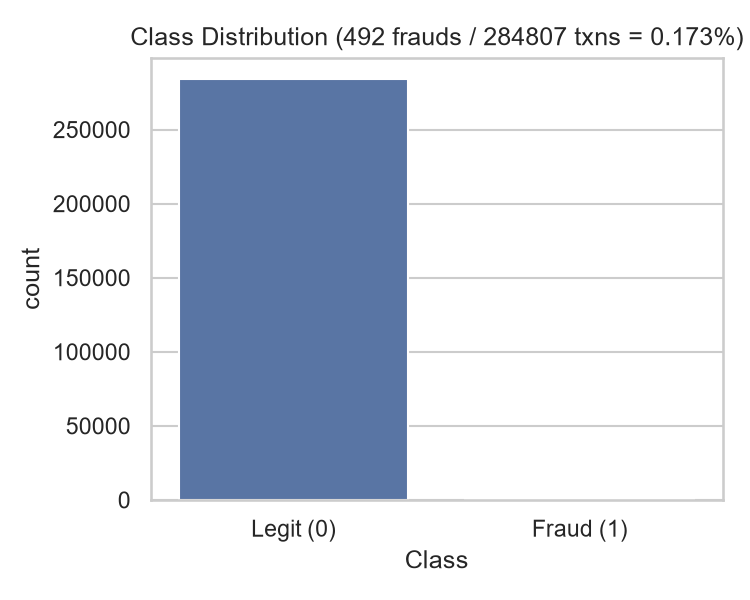
\includegraphics[width=0.55\textwidth]{01_class_distribution.png}
      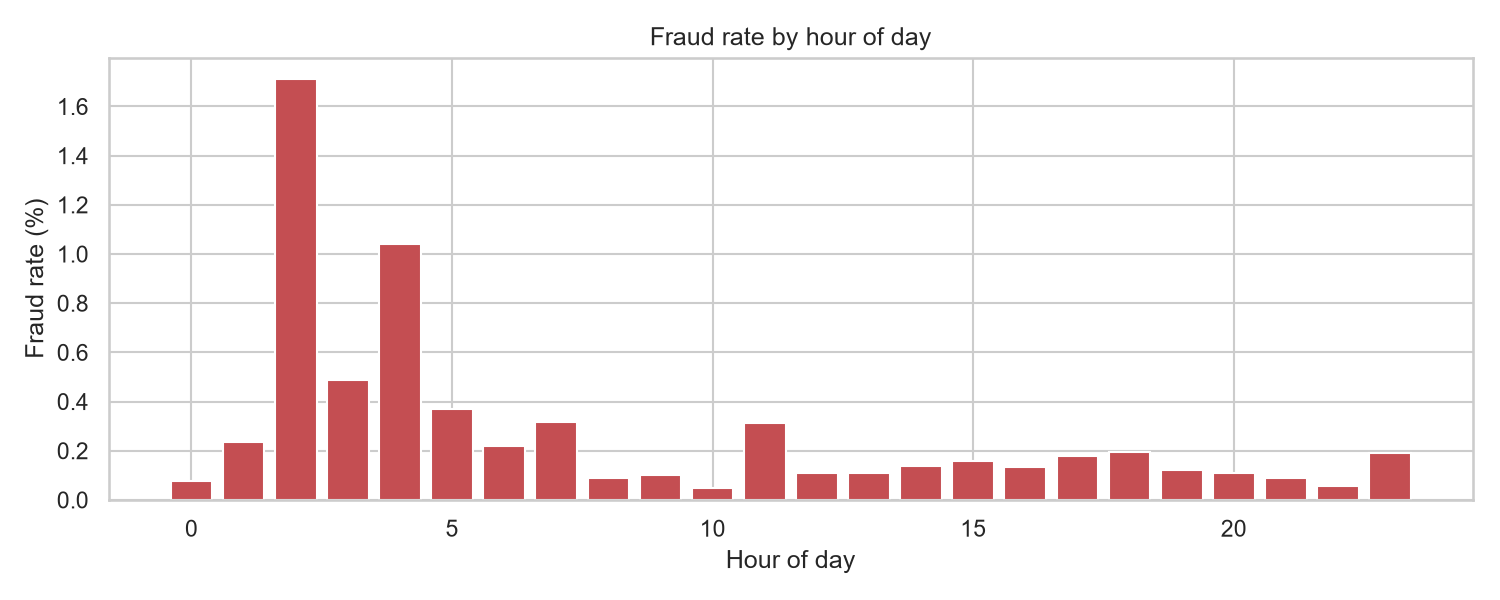
\includegraphics[width=0.42\textwidth]{03_fraud_rate_by_hour.png}
      \caption{\textbf{Left:} the 578:1 class imbalance --- the central difficulty of the task.
            \textbf{Right:} fraud rate by hour peaks around 02:00--04:00 at up to ten times the
            daily average, justifying time features and a chronological split.}
\end{figure}

\textbf{Key exploratory findings.}
(i) No missing values anywhere.
(ii) Fraud amounts skew small (median EUR 9.25 vs.\ EUR 22) yet have a heavier upper tail
relative to their count --- motivating the log transform.
(iii) The features most correlated with the label are $V17, V14, V12, V10$ (negatively) and
$V11$ (positively); no single feature separates the classes, which leaves room for non-linear
models. These observations become the ground truth against which the SHAP explanations of
Section~\ref{sec:shap} are later compared.

% ============================================================================
\section{A taxonomy of model families}\label{sec:taxonomy}
% ============================================================================

This section introduces every family used in the study, building from simplest to most
complex. Table~\ref{tab:families} at the end summarises where each of our 18 trained
architectures belongs.

\subsection{Linear models}
\term{Logistic Regression} fits
$\hat{p} = \sigma(\mathbf{w}^{\top}\mathbf{x} + b)$ where $\sigma$ is the logistic function:
a single weighted vote over features. It is fast, interpretable, and surprisingly hard to beat
when signal is mostly additive. \term{Linear SVM} draws the maximum-margin separating hyperplane
instead of maximising likelihood; empirically it lands near logistic regression here
(PRAUC 0.747 vs 0.738). Both define the \emph{linear ceiling} of the dataset.

\subsection{Probabilistic baseline: Naive Bayes}
\term{Gaussian Naive Bayes} applies Bayes' rule assuming features are independent given the
class. PCA components are uncorrelated \emph{linearly}, but independence still fails badly:
NB scores only $\approx 0.08$ PR-AUC, a reminder that a strong assumption can be worse than no
model when it is violated.

\subsection{Decision trees}
A \term{decision tree} recursively partitions feature space with axis-aligned questions
(``is $V14 < c$?''). A single unpruned tree overfits noise: ours reaches only 0.405 PR-AUC.
Trees are weak alone but are the building blocks of the strongest classical families below.

\subsection{Ensemble methods: many weak learners, one strong committee}
\term{Bagging} (bootstrap aggregation) trains many deep trees on random resamples and averages
them --- variance cancels out. \textbf{Random Forest}~\cite{breiman2001} adds extra randomness
by restricting each split to a random feature subset; it is our overall champion.

\term{Gradient boosting} instead builds trees \emph{sequentially}, each new tree fitting the
residual errors of the current ensemble. Modern implementations --- \textbf{XGBoost}~\cite{chen2016},
\textbf{LightGBM}~\cite{ke2017} (histogram-based splits), and \textbf{CatBoost}~\cite{prokhorenkova2018}
(ordered boosting, robust handling of categorical variables) --- dominate tabular benchmarks.
Their weakness discovered here: blindly setting the positive-class weight to the imbalance ratio
($519$) makes boosting predict almost everything as fraud (Section~\ref{sec:weightab}).

\term{Stacking / voting} combines \emph{different} families: our best deep ensemble averages the
probabilities of a forest, an MLP and an LSTM (0.785). Diversity across families is what pays
off; averaging five LSTMs that differ only in random seed does not (0.775).

\subsection{Neural networks}
All neural nets share the same atom: a \term{layer} computes
$\mathbf{h}' = \phi(W\mathbf{h} + \mathbf{b})$ with a non-linearity $\phi$ (ReLU etc.).
Stacking layers lets the network compose simple features into complex ones.

\begin{description}[leftmargin=1.4em, style=nextline]
      \item[MLP / DNN (feed-forward).] Fully connected layers read one transaction at a time.
            Our MLP (128-64-32 units) scores 0.775; doubling depth and width (DNN, 512-256-128-64
            with batch normalisation) changes nothing (0.7752) --- depth buys nothing on 32
            PCA features.
      \item[Autoencoder.] An encoder compresses legitimate transactions to a 16-dimensional code
            and a decoder reconstructs them; frauds reconstruct poorly, so reconstruction error
            becomes an anomaly score. Trained without labels it reaches ROC-AUC 0.94 but only
            0.584 PR-AUC: ignoring labels costs ranking precision exactly where fraud systems
            need it.
      \item[RNN / LSTM.] Recurrent networks read \emph{sequences}, carrying a hidden state across
            steps; the LSTM's gating cells remember long-range patterns. Feeding sliding windows
            of 8 consecutive transactions lifts performance to 0.780 --- temporal context is real
            signal. Making it bidirectional (BiLSTM, reading forwards and backwards) adds nothing
            (0.781): fraud evidence is causal, not symmetric.
      \item[Transformers.] Replace recurrence with \term{self-attention}, letting every element
            weigh every other element in parallel~\cite{vaswani2017}. \textbf{FT-Transformer}
            applies this to tabular rows (each feature becomes a token); at 0.681 it loses to
            boosting and even to the plain MLP --- attention overhead is unjustified on 32 numeric
            features, consistent with recent tabular-DL studies.
      \item[GANs.] Generative Adversarial Networks~\cite{goodfellow2014} pit a Generator (creates
            fake samples from noise) against a Discriminator (real vs.\ fake) until fakes become
            statistically indistinguishable. We train one on the minority class and use it to
            synthesise frauds (Section~\ref{sec:imbalance}).
\end{description}

\subsection{Graph neural networks}
When entities are linked (card---merchant---device), data forms a \term{graph}
$G=(V,E)$, and \term{message passing} updates each node from its neighbours:
$\mathbf{h}_v' = \mathrm{UPDATE}\big(\mathbf{h}_v,\ \mathrm{AGG}\{\mathbf{h}_u : u \in \mathcal{N}(v)\}\big)$.
\textbf{GraphSAGE}~\cite{hamilton2017} samples a fixed number of neighbours and aggregates
(mean/max/pool); \textbf{GAT}~\cite{velickovic2018} learns attention weights over neighbours.
Crucially, ULB has \emph{no entity identifiers}, so our graph connects each transaction to its
$k{=}10$ nearest neighbours in feature space --- a similarity surrogate. SAGE still reaches
0.756, but attention (GAT, 0.745) adds nothing: there is no true relational structure to attend
over. Optuna's choice of a \emph{single} SAGE layer confirms over-smoothing --- two rounds of
averaging near-identical neighbours blurs discriminative detail.

\begin{table}[h]
      \centering\small
      \caption{Where every trained architecture sits in the taxonomy.}
      \label{tab:families}
      \begin{tabularx}{\textwidth}{llXl}
            \toprule
            \textbf{Family} & \textbf{Model} & \textbf{One-line idea} & \textbf{Best PRAUC}\\
            \midrule
            Linear & LogReg / LinearSVC & weighted vote / max-margin hyperplane & 0.738 / 0.747\\
            Probabilistic & GaussianNB & Bayes rule + independence assumption & 0.079\\
            Tree & DecisionTree & recursive if-else partitioning & 0.405\\
            Bagging & RandomForest & averaged de-correlated trees & \textbf{0.795}\\
            Boosting & XGBoost / LightGBM / CatBoost & sequential residual fitting & 0.777 / 0.775 / 0.783\\
            Feed-forward NN & MLP / DNN & composed dense layers & 0.775 / 0.775\\
            Autoencoder & AE & reconstruction-error anomaly score & 0.584\\
            Recurrent NN & LSTM / BiLSTM & gated state over 8-step windows & 0.780 / 0.781\\
            Transformer & FT-Transformer & self-attention over feature tokens & 0.681\\
            GAN augmentation & GAN + any model & adversarially generated minority samples & 0.783 (CatB)\\
            Graph NN & GraphSAGE / GAT & neighbour message passing & 0.756 / 0.745\\
            Stacked ensemble & RF+MLP+LSTM & average of diverse families & 0.785\\
            \bottomrule
      \end{tabularx}
\end{table}

% ============================================================================
\section{Handling class imbalance}\label{sec:imbalance}
% ============================================================================

Seven strategies were compared, all applied to the \emph{training partition only}:

\begin{enumerate}[leftmargin=*]
      \item \textbf{raw} --- do nothing; establishes each model's floor.
      \item \textbf{class weighting} --- multiply the positive class's loss contribution by a
            weight $w$. The naive choice $w = n_{\text{neg}}/n_{\text{pos}} \approx 519$ can be
            destructive; we select $w$ on the validation grid
            $\{1, 4, 16, \sqrt{r}, 64, r\}$ (with $r$ the imbalance ratio).
      \item \textbf{RUS} --- random undersampling deletes majority rows until classes are even.
            Cheap, but discards $99\%$ of the data (only 768 training rows remain).
      \item \textbf{SMOTE}~\cite{chawla2002} --- Synthetic Minority Over-sampling TEchnique:
            new fraud points are interpolated between neighbouring minority samples.
      \item \textbf{SMOTE-ENN}~\cite{batista2004} --- SMOTE followed by Edited Nearest Neighbours
            cleaning, which removes both noisy synthetics and borderline majorities.
            This \emph{hybrid} is the strongest classical recipe.
      \item \textbf{GAN oversampling} --- a generator adversarially trained on the 384 training
            frauds produces synthetic ones; strong for CatBoost and LightGBM, harmful for
            neural nets and linear models.
      \item \textbf{anomaly framing} --- train only on legitimate data (autoencoder) and flag
            large reconstruction error; requires no labels but wastes the labels we have.
\end{enumerate}

% ============================================================================
\section{Evaluation methodology}\label{sec:protocol}
% ============================================================================

\textbf{Split.} Chronological: earliest $70\%$ train (384 frauds), next $15\%$
validation (56 frauds), latest $15\%$ test (52 frauds). Table~\ref{tab:window} states the
window explicitly, because the honesty of every later claim depends on it.

\begin{table}[h]
      \centering\small
      \caption{The chronological window. ULB spans exactly $48$ hours; the last training
      transaction and the first test transaction are $5.11$~hours apart, and the test window is
      $5.96$~hours long.}
      \label{tab:window}
      \begin{tabular}{lccccc}
            \toprule
            Split & Window (h) & $n$ & Frauds & Fraud rate & Mean amount\\
            \midrule
            Train & $0.00$--$36.92$ & 199{,}364 & 384 & $0.193\%$ & $89.77$\\
            Validation & $36.92$--$42.04$ & 42{,}721 & 56 & $0.131\%$ & $97.52$\\
            Test & $42.04$--$48.00$ & 42{,}722 & 52 & $0.122\%$ & $72.54$\\
            \bottomrule
      \end{tabular}
\end{table}

Two things follow. First, the distribution genuinely moves inside these 48 hours: the fraud
prior falls by $37\%$ relative from train to test ($0.193\%\to0.122\%$) and the mean
transaction amount falls by $19\%$. Second, the window contains two full day--night cycles with
a $35.5\times$ ratio between the peak and trough hourly fraud rates (02:00 peaks at $1.71\%$).
Shuffling destroys both structures, which is the mechanism behind the inflation measured in
Section~\ref{sec:splittab}.

\textbf{Tuning discipline.} Every adaptive choice uses the validation set exclusively:
decision thresholds (max-$F_1$ point of the validation PR curve, frozen thereafter),
class-weight grids, early-stopping epochs, and all Optuna searches (objective =
validation PR-AUC, TPE sampler, seed 42). The test set is scored exactly once per
configuration.

\textbf{Metrics.} Confusion-matrix counts (TP/FP/FN/TN), precision, recall, $F_1$,
Matthews Correlation Coefficient (robust to imbalance), ROC-AUC (reported but known to be
optimistic here), and \textbf{PR-AUC} --- the area under precision versus recall --- as the
primary metric, following the dataset authors' recommendation.

\textbf{Uncertainty.} With 52 test frauds, metrics wobble substantially. We estimate this with
a \term{stratified bootstrap}: resample frauds and legits separately, with replacement,
$1{,}000$ times; recompute PR-AUC per replicate; report the 2.5th--97.5th percentile interval
(Efron~\cite{efron1979}). Overlapping intervals mean two models cannot be told apart on this
data.

% ============================================================================
\section{Results}
% ============================================================================

\subsection{Head-to-head against the protocol-matched study}\label{sec:headtohead}
Sang~\cite{eai2026} reports a chronological ULB split ($187{,}972$ train / $39{,}873$
validation / $56{,}962$ test; 368 / 49 / 75 frauds) with an Optuna-tuned, cost-sensitive
XGBoost and an $F_1$-optimal validation threshold --- the same protocol shape used here.
Table~\ref{tab:h2h} places the two side by side.

\begin{table}[h]
      \centering\small
      \caption{The only protocol-matched comparison available: chronological ULB, both studies
      selecting the decision threshold by validation $F_1$.}
      \label{tab:h2h}
      \begin{tabularx}{\textwidth}{Xll}
            \toprule
            & Sang 2026~\cite{eai2026} & This work\\
            \midrule
            Model & Optuna XGBoost (cost-sensitive) & RF + SMOTE-ENN\\
            PR-AUC & 0.7902 & \textbf{0.7947}\\
            Precision & 0.8636 & \textbf{0.975}\\
            Recall & \textbf{0.7600} & 0.750\\
            $F_1$ & 0.8085 & \textbf{0.848}\\
            FP / FN & 9 / 18 & \textbf{1 / 13}\\
            False positives per $10^6$ legitimate & 158 & \textbf{23}\\
            Test frauds & 75 & 52\\
            \bottomrule
      \end{tabularx}
\end{table}

The two PR-AUC figures differ by $0.0045$, roughly a fifth of what a single transaction is worth
on this test set (Section~\ref{sec:boot}) --- they are the same number. The operating point
differs more substantially: this study trades one point of recall for a seven-fold reduction in
false-alarm rate, which for a fraud-review queue is the more consequential axis.

Three further points from that paper corroborate results derived independently here. First, it
measures the protocol gap on the same model at $0.8815 - 0.7902 = +0.0913$, larger than the
$+0.035$ mean measured in Section~\ref{sec:splittab}, which supports treating our figure as a
floor. Second, its Tables~4 and~5 hold PR-AUC fixed at $0.8815$ and $0.7902$ across three very
different thresholds, confirming that threshold calibration cannot alter a ranking metric --- so
the $0.7809 \to 0.8815$ gain it reports is attributable to hyperparameter search alone. Third,
it independently reaches this study's framing of the dataset's horizon, describing the
$48$-hour window as ``a short-horizon chronological validation rather than a full concept-drift
analysis.'' Its SHAP ranking ($V14, V4, V10, V12, V8$) also overlaps ours in four of five
positions.

\subsection{Robustness: replicating on the published split}\label{sec:sangrep}
The comparison in Section~\ref{sec:headtohead} confounds two things: the split fractions differ
($70/15/15$ against $66/14/20$) and the model families differ (Random Forest against XGBoost).
A replication check was registered in advance --- question, configurations and interpretation
fixed in \code{reports/PREREGISTRATION\_sang\_split.md}, committed before the experiment was
run, so the ordering is verifiable from the repository history rather than asserted. Sang's
partition reproduces exactly from the public CSV: $66/14/20$ on time-sorted, non-deduplicated
rows yields $187{,}972 / 39{,}873 / 56{,}962$ with $368 / 49 / 75$ frauds, matching the paper
to the unit.

\begin{table}[h]
      \centering\small
      \caption{Pre-registered replication on Sang's exact chronological partition. Standard
      error at 75 test frauds is $\approx0.042$. Ledger:
      \code{reports/results\_sang\_split.csv}.}
      \label{tab:sangrep}
      \begin{tabularx}{\textwidth}{Xllll}
            \toprule
            Configuration & $70/15/15$ & $66/14/20$ & $\Delta$ split & vs $0.7902$\\
            \midrule
            XGBoost + class weight & 0.7688 & 0.8055 & $+0.0367$ & $+0.0153$ ($0.37$ SE)\\
            XGBoost + SMOTE-ENN & 0.7766 & 0.8102 & $+0.0336$ & $+0.0200$ ($0.48$ SE)\\
            RF + SMOTE-ENN & 0.7947 & 0.8224 & $+0.0276$ & $+0.0322$ ($0.77$ SE)\\
            \bottomrule
      \end{tabularx}
\end{table}

\textbf{Outcome one: replication, not improvement.} XGBoost with validation-selected class
weighting --- the closest analogue to Sang's cost-sensitive XGBoost, since neither uses
synthetic resampling --- reaches $0.8055$ against the published $0.7902$. That is $0.37$
standard errors. At the $F_1$-optimal threshold it recovers exactly the same 57 of 75 frauds
that paper reports (identical FN${}=18$), with 5 false positives rather than 9. Under the
pre-registered reading this is an independent replication; the margin is far too small to claim
an improvement, and no such claim is made. \emph{The primary protocol of this report remains
$70/15/15$, and the figures in Table~\ref{tab:sangrep} do not replace any headline result.}
Promoting the more favourable of two splits would be exactly the selection effect quantified in
Section~\ref{sec:litcmp}.

\textbf{Outcome two, and the more consequential one: split fractions are a first-order
choice.} Changing only the fractions --- same chronological protocol, same data, same models,
same code --- shifted PR-AUC by $+0.033$ on average. The random-versus-chronological inflation
measured in Section~\ref{sec:splittab} is $+0.035$. \emph{Choosing $20\%$ rather than $15\%$ as
the test tail moves the number about as much as abandoning chronological evaluation
altogether.} Part of the mechanism is visible in the windows: the $66/14/20$ test partition
begins $1.7$ hours earlier and carries a higher fraud prevalence ($0.1317\%$ against
$0.1217\%$), and average precision is bounded below by the positive rate. The remainder is that
a $75$-fraud window and a $52$-fraud window are simply different samples of a non-stationary
process.

The implication is uncomfortable and worth stating plainly: this report's own headline of
$0.795$ is conditioned on a $15\%$ tail, and a defensible alternative choice would have
produced $0.822$. That is a further argument against reading any of these numbers as a ranking.

\subsection{Leaderboard}
Table~\ref{tab:leaderboard} lists the top configurations of all 72 time-split runs.
The full ledger is \code{reports/results\_classical.csv}.

\begin{table}[h]
      \centering\small
      \caption{Top 15 of 72 runs (test set, chronological).}
      \label{tab:leaderboard}
      \begin{tabular}{llcccccc}
            \toprule
            \# & Model + strategy & PR-AUC & $F_1$ & Prec. & Rec. & FP & FN\\
            \midrule
            1 & Random Forest + SMOTE-ENN & \textbf{0.795} & 0.848 & 0.975 & 0.750 & 1 & 13\\
            2 & Random Forest + SMOTE & 0.790 & 0.848 & 0.975 & 0.750 & 1 & 13\\
            3 & RF+MLP+LSTM stack & 0.785 & 0.835 & 0.974 & 0.731 & 1 & 14\\
            4 & Random Forest + class weight & 0.784 & 0.788 & 0.830 & 0.750 & 8 & 13\\
            5 & CatBoost + GAN & 0.783 & 0.848 & 0.975 & 0.750 & 1 & 13\\
            6 & BiLSTM + class weight & 0.781 & 0.839 & 0.951 & 0.750 & 2 & 13\\
            7 & LSTM + class weight & 0.780 & 0.813 & 0.949 & 0.712 & 2 & 15\\
            8 & XGBoost + SMOTE-ENN & 0.777 & 0.813 & 0.886 & 0.750 & 5 & 13\\
            9 & LightGBM + GAN & 0.775 & 0.822 & 0.974 & 0.712 & 1 & 15\\
            10 & LSTM ensemble (5 seeds) & 0.775 & 0.831 & 1.000 & 0.712 & 0 & 15\\
            11 & MLP + raw & 0.775 & 0.809 & 0.973 & 0.692 & 1 & 16\\
            \bottomrule
      \end{tabular}
\end{table}

The champion flags 39 of 52 frauds while raising a single false alarm among 42{,}722
transactions --- production-grade precision at useful recall.

\subsection{Imbalance-strategy ablation}
Across the four boosted/forest models the ordering predicted by Ahmed et al.~\cite{ahmed2025}
reproduces exactly: \emph{hybrid $>$ oversampling $>$ weighting $>$ raw}. GAN synthesis is the
top strategy for CatBoost (0.783) and rescues LightGBM, but hurts linear models badly
(LogReg drops to 0.568): synthetic-data gains are model-dependent, never universal.

\subsection{Class-weight ablation}\label{sec:weightab}
Keeping the classic fixed weight $r \approx 519$ as a visible control row, validation-selected
weights improve every boosted model: XGBoost $0.761 \to 0.769$ (chose $w{=}16$),
CatBoost $0.762 \to 0.765$ ($\sqrt{r}$), and rescue LightGBM from total collapse
($0.009 \to 0.537$, with validation rejecting any weighting at all). Optuna later searched the
weight continuously and picked $4.1$--$172$ --- two independent mechanisms agreeing that the
textbook ratio is far too aggressive.

\subsection{Random-split ablation: quantifying leakage}\label{sec:splittab}
Re-running one configuration per tier under the shuffled protocol used by most papers:

\begin{table}[h]
      \centering\small
      \caption{Chronological vs shuffled split (same models, same data).}
      \label{tab:splits}
      \begin{tabular}{lccc}
            \toprule
            Configuration & Time split & Random split & Inflation\\
            \midrule
            CatBoost + GAN & 0.780 & 0.840 & $+0.060$\\
            MLP raw & 0.779 & 0.827 & $+0.047$\\
            XGBoost + SMOTE-ENN & 0.777 & 0.810 & $+0.034$\\
            RandomForest + SMOTE-ENN & 0.795 & 0.812 & $+0.017$\\
            LSTM + class weight & 0.780 & 0.797 & $+0.016$\\
            GraphSAGE + weight & 0.739 & 0.695 & $-0.044$\\
            \bottomrule
      \end{tabular}
\end{table}

Shuffling inflates five of six configurations --- up to $+0.06$ for the synthetic-data
pipeline, whose fabricated frauds land next to their real neighbours in the test fold.
Our measured shuffled numbers ($0.80$--$0.84$) move into the band where the published
random-split literature sits: a large share of the historical benchmark gap is
\emph{protocol, not model quality}. GraphSAGE is the instructive exception --- shuffling
scrambles the temporal coherence its neighbourhoods relied upon.

\subsection{Statistical uncertainty}\label{sec:boot}
Stratified-bootstrap intervals (Table~\ref{tab:boot}; Figure~\ref{fig:boot}) are wide ---
widths of $0.20$--$0.24$ --- and \emph{every pairwise comparison overlaps}: at 52 test frauds
no two models are statistically separable. Claims like ``tuned RF beats untuned RF''
($0.7936$ vs $0.7947$) are correctly described as ties. Run-to-run variance is family-dependent
and small: the tree tiers reproduce bit-exactly, MLP and LSTM vary by $\approx 0.01$, and
GraphSAGE by $\approx 0.02$ across three same-configuration invocations ($0.724$--$0.756$). An earlier
draft of this section reported a $0.13$-wide ``GraphSAGE instability''; that was an artifact of
a harness bug (its $k$-NN graphs were built on unscaled features, where \code{Amount} owns
$99.9\%$ of the Euclidean distance budget and the informative $V$-features are effectively
discarded) and has been retracted. A separate asymmetry is worth noting: full-batch SAGE takes
at most 40 optimizer steps versus $\approx 5{,}850$ for mini-batched GAT. Forcing SAGE to train
the full 300 steps with early stopping disabled \emph{degrades} test PR-AUC to $0.707$, and
the trajectory says why: validation AP keeps improving ($0.837$ at step 20 to $0.845$ at step
250) while test AP falls ($0.756$ to $0.673$). The extra steps buy a tighter fit to the
train/validation era --- chronologically adjacent windows --- at the cost of extrapolating to
the later test window. That is temporal drift, not over-smoothing: depth is fixed at two layers
throughout. So the budget gap does not flatter SAGE, and the GAT comparison stands: the
better-trained model only ties. Probe: \texttt{python -m src.models.probe\_sage\_budget}. This
reframes the deliverable: the enduring value is the protocol and the ablation evidence, not
rank order.

\begin{table}[h]
      \centering\small
      \caption{Stratified-bootstrap 95\% CIs ($1{,}000$ replicates).}
      \label{tab:boot}
      \begin{tabular}{lccl}
            \toprule
            Config & PR-AUC & 95\% CI & width\\
            \midrule
            RF + SMOTE-ENN & 0.795 & [0.692, 0.888] & 0.196\\
            CatBoost + GAN & 0.780 & [0.674, 0.880] & 0.206\\
            LSTM + weight & 0.780 & [0.669, 0.879] & 0.210\\
            MLP raw & 0.779 & [0.671, 0.877] & 0.206\\
            XGBoost + SMOTE-ENN & 0.777 & [0.669, 0.880] & 0.211\\
            GraphSAGE + weight & 0.724 & [0.601, 0.837] & 0.236\\
            \bottomrule
      \end{tabular}
\end{table}

\textbf{How much is one transaction worth?} The bootstrap says the intervals are wide; a direct
perturbation of the champion's saved score vector says why. Removing any single test fraud
(52 variants) moves PR-AUC over a range of $0.020$; promoting the worst-ranked test fraud to the
top of the ranking moves it $+0.020$; demoting the best-ranked fraud to the bottom moves it
$-0.020$. \emph{One transaction is worth roughly $\pm0.020$ PR-AUC.} Any difference below about
$0.02$ on this test set is therefore arithmetic noise rather than evidence --- a rule this report
applies to its own leaderboard and, in Section~\ref{sec:litcmp}, to comparisons against other
papers.

\begin{figure}[h]
      \centering
      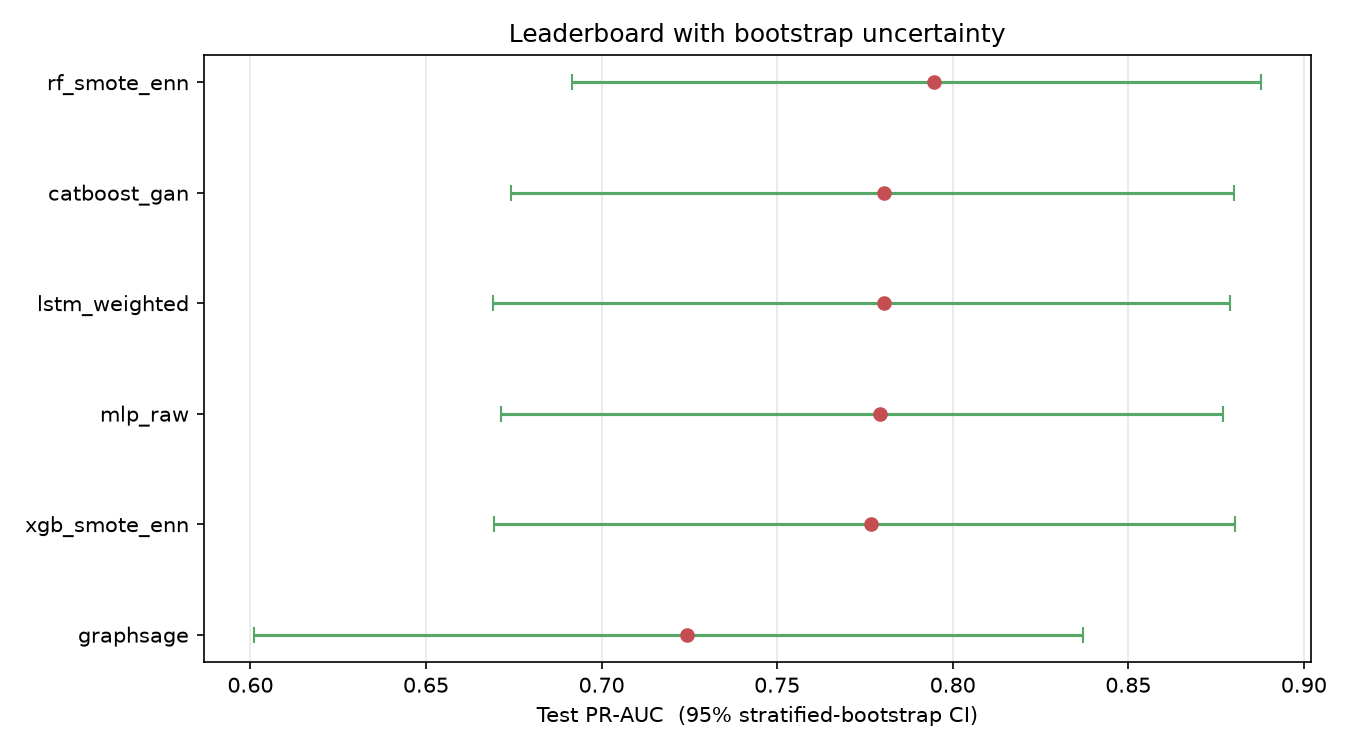
\includegraphics[width=0.85\textwidth]{bootstrap_ci.png}
      \caption{Forest plot: point estimates with stratified-bootstrap 95\% intervals.
            Complete overlap everywhere.}
      \label{fig:boot}
\end{figure}

% ============================================================================
\section{Explainability: SHAP}\label{sec:shap}
% ============================================================================

\term{SHAP} (SHapley Additive exPlanations)~\cite{lundberg2017} imports Shapley values from
cooperative game theory: treat features as players and the prediction as the payout, then pay
each feature its average marginal contribution over all orderings. Unlike generic importances,
SHAP yields a signed contribution \emph{per transaction}: ``low $V12$ added $+\delta$ to this
transaction's fraud logit.''

Applying TreeExplainer to the champion over 3{,}052 test rows (all 52 frauds plus a 3{,}000-row
legitimate sample):

\begin{figure}[h]
      \centering
      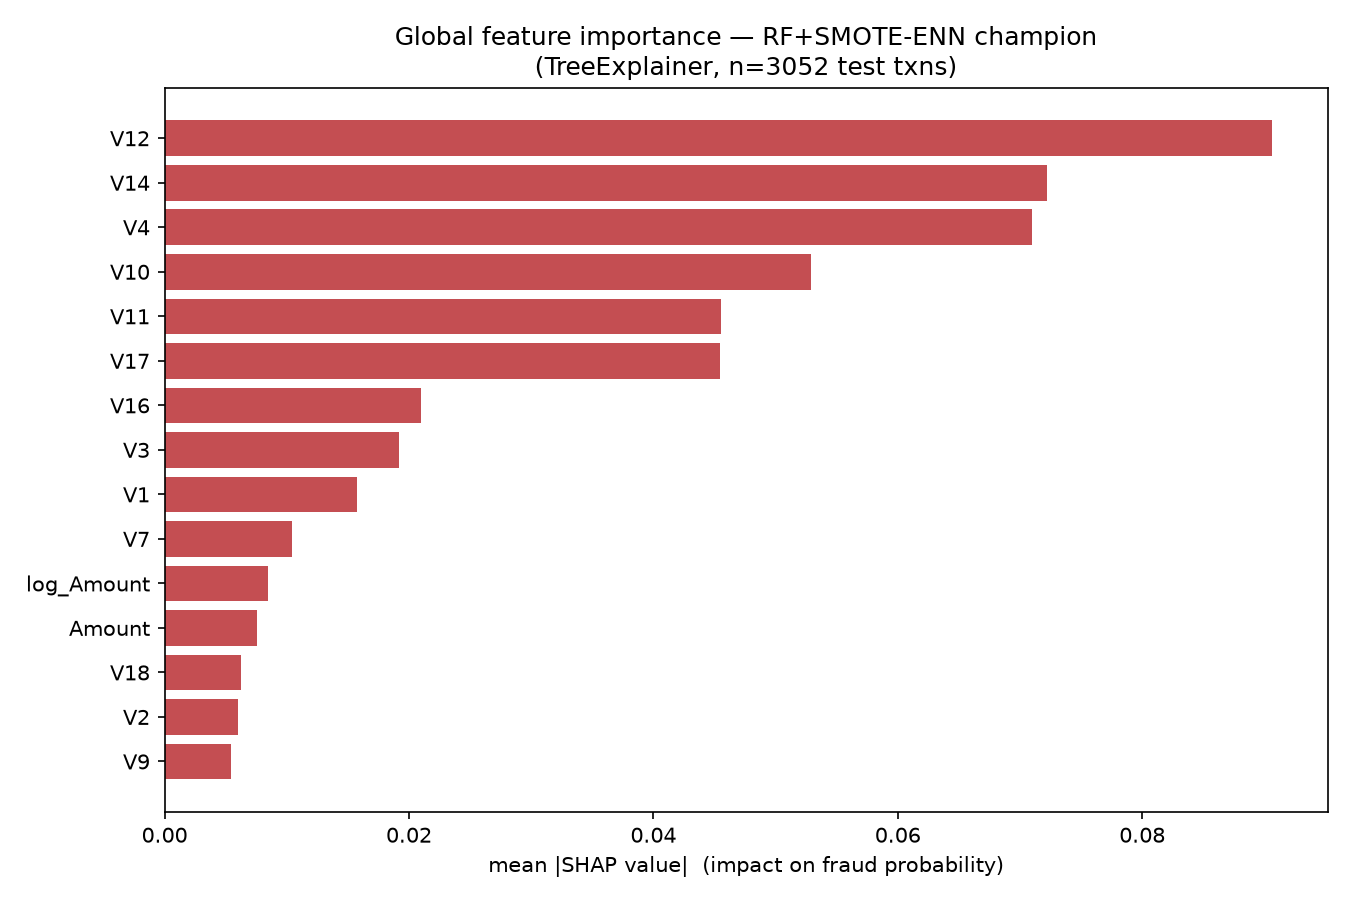
\includegraphics[width=0.72\textwidth]{shap_global_importance.png}\\[0.3cm]
      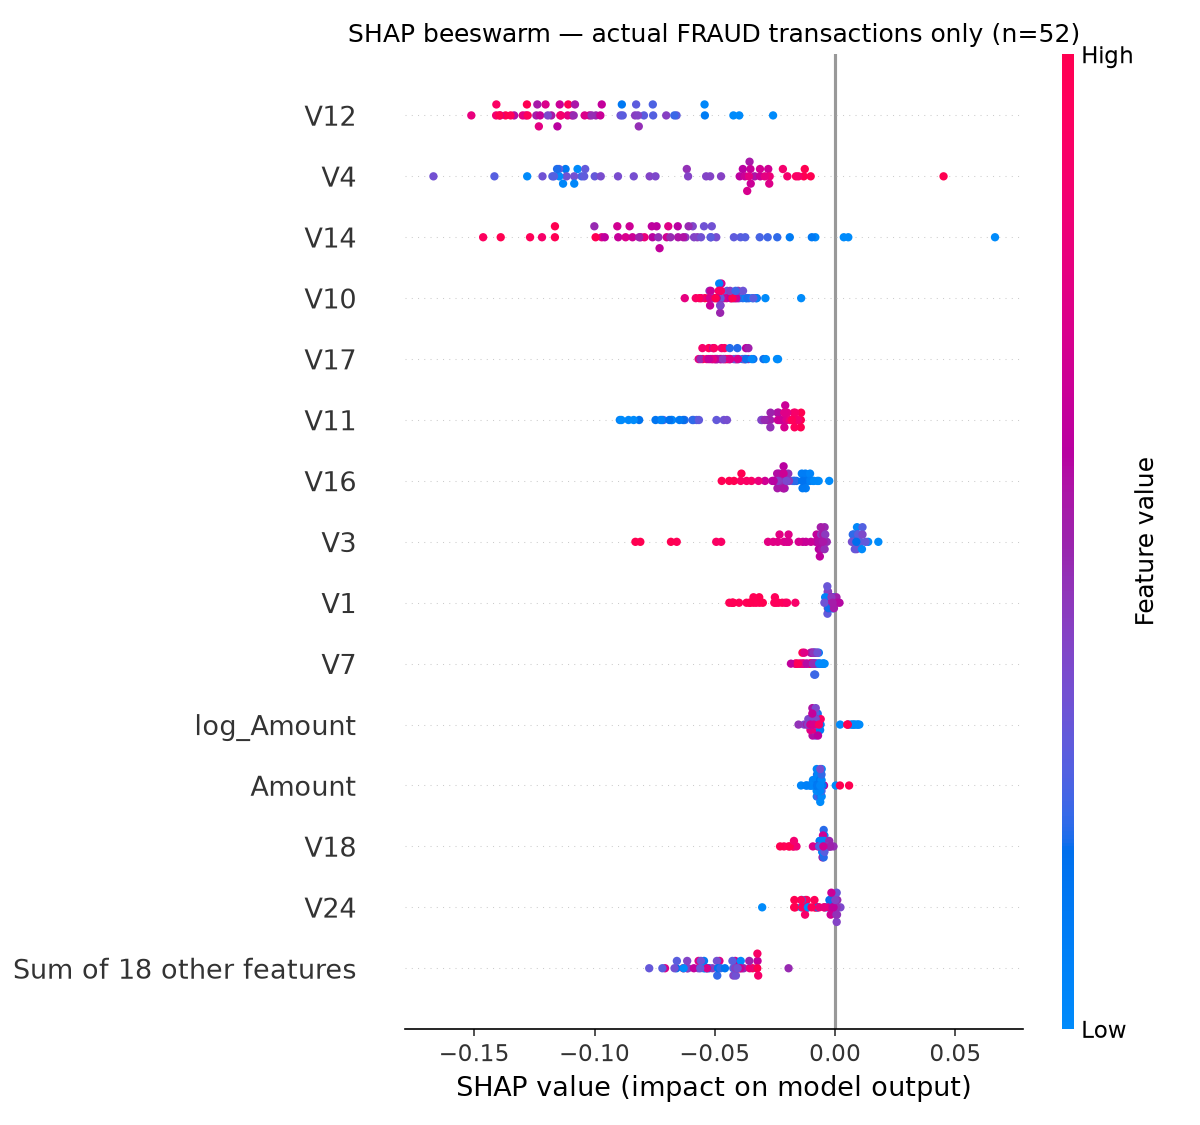
\includegraphics[width=0.66\textwidth]{shap_beeswarm_fraud.png}
      \caption{Global SHAP importance (top) and beeswarm over actual fraud transactions
            (bottom): red = high feature value, blue = low; rightward = pushes toward fraud.}
\end{figure}

The ranking --- $V12, V14, V4, V10, V11, V17$ --- matches the Phase-1 correlation analysis
feature-for-feature \emph{and} sign-for-sign ($V12/V14/V10/V17$ low $\to$ fraud,
$V11$ high $\to$ fraud, small amounts $\to$ fraud). Two independent methods agreeing on both
axes is strong evidence the model learned genuine structure rather than artifacts. A per-transaction
waterfall (\code{shap\_waterfall\_example.png}) powers the
``why flagged'' view of the demo application.

% ============================================================================
\section{Comparison with the literature}
% ============================================================================
\label{sec:litcmp}

\begin{table}[h]
      \centering\small
      \caption{Published reference points and this work. PR-AUC (average precision) unless
      otherwise noted.}
      \label{tab:lit}
      \begin{tabularx}{\textwidth}{lXl}
            \toprule
            Source & Setting & Best PR-AUC\\
            \midrule
            KAIS 2026~\cite{kais2026} & private bank data, random CV & 0.9879\\
            EAI ISMLA 2026~\cite{eai2026} & ULB, optimised XGBoost, random split & 0.8815\\
            IJSSE 2025~\cite{ijsse2025} & ULB, SMOTE + RF / XGBoost, random split & 0.871 / 0.867\\
            Anand \& Chakrabarty 2025~\cite{anand2025} & ULB, LSTM ensemble, random split & 0.8269\\
            HG-AE~\cite{hgae2024} & \emph{relational} graph (cardholder/merchant/txn) & $\approx$0.89\\
            HGNN + attention~\cite{hgnn2025} & IEEE-CIS, \emph{not} ULB & ROC-AUC only\\
            \midrule
            \textbf{This work} & \textbf{ULB, chronological split} & \textbf{0.795}\\
            \textbf{This work} & \textbf{ULB, shuffled (their protocol)} & \textbf{0.840}\\
            \bottomrule
      \end{tabularx}
\end{table}

\subsection{Only the shuffled arm is comparable}
Nearly all published ULB results use a random or stratified split. The one exception we located
is Sang~\cite{eai2026}, which reports a chronological ULB PR-AUC of $0.7902$ for an
Optuna-tuned cost-sensitive XGBoost; our champion reaches $0.7947$ at roughly one-seventh the
false-positive rate (Section~\ref{sec:headtohead}). A pre-registered replication on that
paper's exact partition (Section~\ref{sec:sangrep}) places our XGBoost $0.37$ standard errors
from its published value. Against every other published figure the
comparison must go through our shuffled arm, where our best configuration reaches $0.840$ and
the tree models reach $0.810$--$0.812$, against $0.867$--$0.8815$ reported.

One asymmetry matters when interpreting that. Our shuffled arm still applies resampling
\emph{inside} the fitted pipeline, so it isolates the effect of destroying temporal ordering and
nothing else. It does not include the far larger inflation available from resampling before the
split. The mean inflation we measure ($+0.035$ across five configurations) is therefore a
\emph{lower bound} on total literature inflation, not an estimate of it.

\subsection{The residual gap is not resolvable at this sample size}
Applying this report's own uncertainty machinery to the cross-paper comparison: the bootstrap
half-width of $0.098$ implies a standard error of $\approx0.050$ at 52 frauds, or $\approx0.042$
rescaled to the 74 frauds of the shuffled test fold. The standard error of a \emph{difference}
between two such single-split estimates is $\approx0.059$. The observed gap --- $0.871$ against
our $0.812$ --- is $0.059$, or \textbf{0.99 standard errors}. Combined with the one-transaction
sensitivity of $\pm0.020$ established above, the entire cross-paper gap is worth roughly three
transactions.

The honest conclusion is the one Section~\ref{sec:boot} reaches for within-study comparisons,
extended one step further: at 52--74 test frauds, \emph{no two ULB PR-AUC figures are separable
--- ours included}. Cross-paper ranking on this dataset is not a meaningful exercise, and the
appropriate response is to report intervals rather than to explain away a difference the data
cannot support.

\subsection{Methodological context, and what the GNN numbers require}
An independent 2025 audit of this literature~\cite{leakage2025} surveys published ULB pipelines
and identifies four recurring flaws: leakage from preprocessing before the split, vague
methodological reporting, inadequate temporal validation, and recall optimisation at precision's
expense. It demonstrates the point by building a deliberately leaky minimal MLP that reaches
$99.9\%$ recall and outperforms far more sophisticated published methods, concluding that proper
evaluation methodology matters more than model complexity. The protocol of
Section~\ref{sec:protocol} was built against all four flaws: resampling is fitted inside the
pipeline on training folds only, every run is logged to a committed ledger, the split is
chronological, and PR-AUC with a validation-frozen threshold is primary with both error types
reported.

The relational-GNN figure of $\approx0.89$~\cite{hgae2024} is obtained on graphs of cardholders,
merchants and transactions. ULB's PCA anonymisation removes every entity identifier, so a
$k$-NN feature-similarity graph is the only construction available: the comparison is one of
\emph{data availability}, not architecture. The frequently cited HGNN-with-attention
work~\cite{hgnn2025} evaluates on IEEE-CIS rather than ULB and reports accuracy and ROC-AUC
rather than PR-AUC, so it is not a ULB reference point at all.

\section{Lessons learned}
% ============================================================================

\begin{enumerate}[leftmargin=*]
      \item \textbf{Hybrid cleaning beats blind synthesis} for tree ensembles
            (SMOTE-ENN $>$ SMOTE $>$ weights $>$ raw).
      \item \textbf{Never assume the textbook class weight.} Validate it; the naive ratio can
            silently destroy a booster.
      \item \textbf{Ensemble diversity must cross families}, not random seeds.
      \item \textbf{Match the architecture to the data's structure:} sequences reward RNNs;
            absent entities starve GNNs; depth starves on wide-but-shallow tabular signal.
      \item \textbf{Report uncertainty.} At 52 positives, everything inside the CI band is a tie.
      \item \textbf{Protocol dominates model choice:} the same models move by $+0.10$ when the
            split leaks.
\end{enumerate}

% ============================================================================
\section{Limitations and future work}
% ============================================================================

\textbf{The two-day window --- and what it does and does not limit.} ULB spans exactly 48 hours,
so the chronological protocol places only $5.11$ hours between the last training transaction and
the first test transaction (Table~\ref{tab:window}). This is the single most important limitation
to state precisely, because it bounds one claim and not another.

What this study claims is an \emph{evaluation-protocol} effect: does shuffling temporally ordered
transactions inflate reported scores? That question is answerable inside 48 hours, because it
concerns whether the evaluation respects causal ordering, not how far the distribution travels.
What this study does \emph{not} claim is a measurement of concept drift or model decay over
deployment timescales; that would require months of data and is out of scope here.

Two observations make the short horizon a conservative choice rather than a weak one. First, the
distribution demonstrably shifts even within the window --- the fraud prior falls $37\%$ relative
across the splits and mean amount falls $19\%$ --- so there is real structure for shuffling to
destroy. Second, the inflation we measure ($+0.016$ to $+0.060$) is obtained across only $5.11$
hours of separation; a deployment gap of weeks or months would be larger, not smaller. The figure
should be read as a floor.

\textbf{Sensitivity to the split fractions.} Section~\ref{sec:sangrep} shows that moving the
chronological cut from $70/15/15$ to $66/14/20$ changes PR-AUC by $+0.033$ on average, a shift
comparable to the random-versus-chronological effect this report is built to measure. The
headline $0.795$ is therefore conditioned on one defensible choice among several, and a
$20\%$ tail would have yielded $0.822$ for the same champion. No result here should be read as
robust to that choice; the ranking-free conclusion of Section~\ref{sec:boot} is the appropriate
one. A fuller treatment would sweep the cut point and report the resulting envelope, which is
left to future work.

\textbf{Other limitations.} Only 52 test frauds, so every confidence interval is wide
($0.20$--$0.24$) and no two models are separable; PCA anonymisation prevents true relational
graphs and business rules; a single dataset from a single 2013 snapshot, with no cross-dataset
replication; GPU search budgets bounded at 25--60 Optuna trials; the GNN tier relies on a
feature-similarity graph that is a proxy for, not an instance of, a real transaction network.

\textbf{Future work.} Replicate the split ablation on an identity-rich, longer-horizon dataset
(IEEE-CIS spans months) to test whether the protocol gap widens as predicted; entity-aware graphs
where cardholder and merchant nodes exist; online and drift-adaptive learning; cost-sensitive
thresholds using real interception costs; probability calibration (Brier score, ECE); repeated
shuffled splits across several seeds, and a sweep of the chronological cut point, to put
intervals on both the inflation estimate and the split-fraction sensitivity; larger
trial budgets and nested resampling for tighter intervals.

\section{Conclusion}
% ============================================================================

We delivered a complete, reproducible fraud-analytics study: eighteen architectures across five
families, seven imbalance strategies, and nine controlled ablations, all under one disciplined
chronological protocol with SHAP explanations and bootstrap uncertainty. The champion
(Random Forest + SMOTE-ENN) achieves production-grade operating characteristics, and the study's
central lesson generalises beyond fraud: \emph{when methodology is held constant, model families
converge; when it varies, it --- not the model --- explains most of what the literature calls
progress.}

% ============================================================================
\begin{thebibliography}{99}\small
\bibitem{dalpozzolo2018} A. Dal Pozzolo, G. Boracchi, O. Caelen, C. Alippi, G. Bontempi.
\emph{Credit Card Fraud Detection: A Realistic Modeling and a Novel Learning Strategy}.
IEEE Trans.\ Neural Networks and Learning Systems, 29(8), 2018.
\bibitem{ahmed2025} K. H. Ahmed, S. Axelsson, Y. Li, A. M. Sagheer.
\emph{A Credit Card Fraud Detection Approach Based on Ensemble Machine Learning Classifier with
Hybrid Data Sampling}. Machine Learning with Applications, 20:100675, 2025.
\bibitem{anand2025} A. Anand, S. Chakrabarty. \emph{Credit Card Fraud Detection and Credit Risk
Analysis: Machine Learning Approaches}. SSRN 5337550, 2025.
\bibitem{kais2026} \emph{AI-based credit card fraud detection: a machine learning approach with
model explainability on real-world data}. Knowledge and Information Systems, 2026.
DOI 10.1007/s10115-026-02773-7. (RF PR-AUC $0.9879\pm0.0008$, XGBoost $0.9874\pm0.0007$;
nine models, four sampling strategies, private and public data.)
\bibitem{eai2026} V. N. T. Sang. \emph{Enhancing Credit Card Fraud Detection under Severe Class
Imbalance using Cost-Sensitive Learning and Threshold Optimization}. EAI Endorsed Transactions on
Intelligent Systems and Machine Learning Applications, Vol.\ 3, 2026 (published 1 June 2026).
(ULB random stratified: XGBoost PR-AUC $0.7809 \to 0.8815$; ULB chronological: $0.7902$.)
\bibitem{hgnn2025} \emph{Detecting Credit Card Fraud via Heterogeneous Graph Neural Networks with
Graph Attention}. arXiv:2504.08183, 2025.
\bibitem{hgae2024} M. T. Singh et al. \emph{Heterogeneous Graph Auto-Encoder for CreditCard Fraud
Detection}. arXiv:2410.08121, 2024.
\bibitem{lundberg2017} S. Lundberg, S.-I. Lee. \emph{A Unified Approach to Interpreting Model
Predictions}. NeurIPS, 2017.
\bibitem{chawla2002} N. V. Chawla et al. \emph{SMOTE: Synthetic Minority Over-sampling Technique}.
Journal of Artificial Intelligence Research, 16, 2002.
\bibitem{batista2004} G. E. A. P. A. Batista et al. \emph{A Study of the Behavior of Several Methods
for Balancing Machine Learning Training Data}. SIGKDD Explorations, 6(1), 2004.
\bibitem{breiman2001} L. Breiman. \emph{Random Forests}. Machine Learning, 45(1), 2001.
\bibitem{chen2016} T. Chen, C. Guestrin. \emph{XGBoost: A Scalable Tree Boosting System}. KDD, 2016.
\bibitem{ke2017} G. Ke et al. \emph{LightGBM: A Highly Efficient Gradient Boosting Decision Tree}.
NeurIPS, 2017.
\bibitem{prokhorenkova2018} L. Prokhorenkova et al. \emph{CatBoost: Unbiased Boosting with
Categorical Features}. NeurIPS, 2018.
\bibitem{vaswani2017} A. Vaswani et al. \emph{Attention Is All You Need}. NeurIPS, 2017.
\bibitem{goodfellow2014} I. Goodfellow et al. \emph{Generative Adversarial Nets}. NeurIPS, 2014.
\bibitem{hamilton2017} W. L. Hamilton, R. Ying, J. Leskovec. \emph{Inductive Representation
Learning on Large Graphs (GraphSAGE)}. NeurIPS, 2017.
\bibitem{velickovic2018} P. Veli\v{c}kovi\'c et al. \emph{Graph Attention Networks}. ICLR, 2018.
\bibitem{gorishniy2021} Y. Gorishniy et al. \emph{Revisiting Deep Learning Models for Tabular Data}.
NeurIPS, 2021.
\bibitem{hochreiter1997} S. Hochreiter, J. Schmidhuber. \emph{Long Short-Term Memory}. Neural
Computation, 9(8), 1997.
\bibitem{leakage2025} \emph{Data Leakage and Deceptive Performance: A Critical Examination of
Credit Card Fraud Detection Methodologies}. arXiv:2506.02703, 2025.

\bibitem{ijsse2025} \emph{Comparative Analysis of Machine Learning Models for Credit Card Fraud
Detection Using SMOTE for Class Imbalance}. International Journal of Safety and Security
Engineering, 15(5), 2025.

\bibitem{efron1979} B. Efron. \emph{Bootstrap Methods: Another Look at the Jackknife}. Annals of
Statistics, 7(1), 1979.
\end{thebibliography}

\appendix
% ============================================================================
\section{Reproducibility}
% ============================================================================

Environment: Python 3.12 virtual environment; PyTorch 2.13.0+cu130 (NVIDIA RTX 5050);
scikit-learn 1.9, XGBoost 3.4, LightGBM 4.7, CatBoost 1.2.10, imbalanced-learn 0.14,
SHAP 0.52, Optuna 4.9. Global seed 42.

\begin{table}[h]
      \centering\small
      \begin{tabularx}{\textwidth}{lX}
            \toprule
            Artifact & Command\\
            \midrule
            Data download & \code{python -m src.data.make\_dataset}\\
            Classical tier & \code{python -m src.models.train\_classical}\\
            Deep tier & \code{python -m src.models.train\_deep}\\
            GNN tier & \code{python -m src.models.train\_gnn}\\
            Ensembles & \code{python -m src.models.train\_ensembles}\\
            Tuning & \code{python -m src.models.tune\_optuna}\\
            Split ablation & \code{python -m src.models.ablation\_random\_split}\\
            Bootstrap CIs & \code{python -m src.models.bootstrap\_ci}\\
            SHAP & \code{python -m src.models.explain\_shap}\\
            Demo app & \code{streamlit run app/streamlit\_app.py}\\
            Final notebook & \code{notebooks/02\_final\_report.ipynb}\\
            \bottomrule
      \end{tabularx}
\end{table}

\section{Glossary}
\begin{description}[leftmargin=1.4em, style=nextline]
      \item[PR-AUC] Area under the precision--recall curve; threshold-free ranking quality for
            imbalanced data. Primary metric throughout.
      \item[MCC] Matthews Correlation Coefficient; a balanced accuracy-like measure that stays
            informative under extreme imbalance.
      \item[Leakage] Any information reaching training that would be unavailable at prediction
            time (future rows, synthetic twins of test points, test-informed tuning).
      \item[Over-smoothing] Degeneration of GNN representations after repeated neighbourhood
            averaging; motivates shallow graphs here.
      \item[stratified bootstrap] Resampling that preserves subgroup sizes (fraud/legit counts)
            so metric replicates remain meaningful.
      \item[pos\_weight / scale\_pos\_weight] Multiplier on the positive class loss term;
            compensates imbalance but must be validated.
\end{description}

\end{document}
